\documentclass[12pt,a4paper]{article}
\usepackage{amsmath}
\usepackage{amsfonts}
\usepackage{amssymb}
\usepackage{polski}
\usepackage{indentfirst}
\usepackage{graphicx}
\usepackage{natbib}
\usepackage{verbatim}
\usepackage{commath}
\usepackage{url}
\usepackage{hyperref}
\usepackage[margin=1in]{geometry}
\usepackage{mathtools}
\DeclarePairedDelimiter\ceil{\lceil}{\rceil}
\DeclarePairedDelimiter\floor{\lfloor}{\rfloor}

\begin{document}

\title{Analiza i Przetwarzanie Dźwięku - Sprawozdanie z projektu 2.}
\author{Szymon Tomulewicz}
\date{17 VI 2020}
\maketitle
\tableofcontents
\newpage

\section{Wprowadzenie\label{sec:wprowadzenie}}
    Celem projektu było stworzenie aplikacji okienkowej, umożliwiającej analizę częstotliwościową sygnałów dźwiękowych. Aplikacja umożliwia rysowanie wykresu sygnału w dziedzinie czasu, rysowanie widma częstotliwościowego, rysowanie spektrogramu oraz rysowanie wykresu częstotliwości krtaniowej.

    \subsection{Aplikacja\label{sec:aplikacja}}
        Aplikacja została wykonana w języku C\#, przy użyciu biblioteki \emph{NAudio} do przetwarzania i analizy plików dźwiękowych, bibliotek \emph{WPF} i \emph{OxyPlot} do stworzenia interfejsu oraz wyświetlania parametrów, a także biblioteki \emph{Math.NET Numerics} do celów obliczeniowych.

        W górnej części interfejsu znajduje się menu umożliwiające wybór pliku do analizy, długości ramki (w próbkach) oraz funkcji okienkowej. Wyświetlany jest także przebieg czasowy wczytanego sygnału. Dolna część interfejsu składa się z zakładek prezentujących różne wykresy - transformatę Fouriera, spektrogram, wykres częstotliwości krtaniowej od czasu, a także cepstrum dla wybranej ramki. Na poniższym rysunku (Rys. \ref{fig:app}) znajduje się przykładowy stan apliakcji po załadowaniu pliku \emph{wav}.

        \begin{figure}[h!]
            \centering
            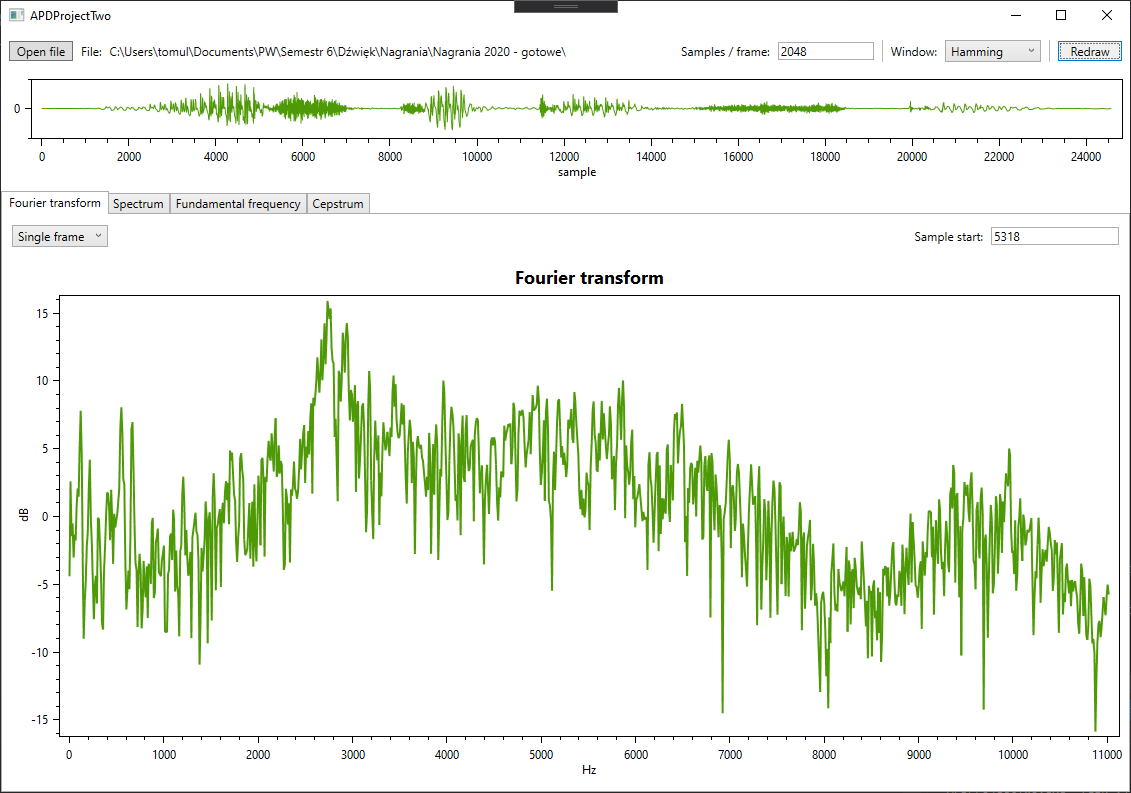
\includegraphics[width=1.0\textwidth]{figures/201_bla_widmo.png}
            \caption{Aplikacja po załadowaniu pliku i wybraniu zakładki \emph{Fourier transform}}
            \label{fig:app}
        \end{figure}

        Wybór rozmiaru ramki i funkcji okienkowej wpływa na wszystkie wykresy, natomiast wybór współczynnika nakładania się ramek wpływa na spektrogram i wykres częstotliwości krtaniowej. Ich wpływ opisany jest w kolejnych sekcjach.

\section{Obliczane wartości i metody\label{sec:wartosci}}
    Wszystkie obliczenia w aplikacji, które są wykonywane na próbkach, używają typów zmiennoprzecinkowych. Parametry opisane w kolejnych sekcjach są obliczane, a następnie zapisywane i wyświetlane w formie wykresów. $N$ występujące we wzorach oznacza zwykle długość ramki w próbkach.

    Na początku wczytywane są wszystkie próbki z pliku, ale analizowane są wyłącznie dla jednego kanału:

    \begin{verbatim}
    // Add samples from single channel to FFT aggregator
    int limit = fftLength * channels + offset;
    for (int n = offset; n < limit; n += channels)
    {
        aggregator.Add(samples[n]);
    }
    \end{verbatim}

    \subsection{Widmo częstotliwości\label{sec:widmo}}
        Do wyznaczenia widma częstotliwości aplikacja używa FFT (z biblioteki \emph{Math.NET Numerics}). Transformata może być wykonana dla całego sygnału. Jeśli ilość próbek w całym sygnale nie mieści się w najbliższej potędze dwójki, jest ``obcinana'':
        \begin{equation*}
            m=\floor*{log_2{N}},
        \end{equation*}
        \begin{equation*}
            N:=2^m.
        \end{equation*}

        Transformata może być również wykonana dla pojedynczej ramki z uwzględnieniem próbki od której ma się rozpoczynać.

        Podczas wykonywania FFT na sygnał nakładana jest jedna z dostępnych funkcji okienkowych

        \begin{itemize}
            \item
                Hamminga:
                \begin{equation*}
                    w(n)=0.54-0.46cos(2\pi\frac{n}{N}), 0 \leq n \leq N.
                \end{equation*}
            \item
                Hanna:
                \begin{equation*}
                    w(n)= 0.5*(1-cos(2\pi\frac{n}{N}), 0 \leq n \leq N.
                \end{equation*}
            \item
                Prostokątna:
                \begin{equation*}
                    w(n)=n,  0 \leq n \leq N.
                \end{equation*}
        \end{itemize}

        Efektem jest wykres widma częstotliwości, którego przykład zaprezentowany jest na Rys. \ref{fig:app}.

    \subsection{Spektrogram\label{sec:spektro}}
        Spektrogram zrealizowany jest poprzez narysowanie na mapie cieplnej wyników FFT liczonych dla kolejnych ramek. Czas jest na osi poziomej, częstotliwości na osi pionowej, natomiast wartość dla danej częstotliwości oznaczany jest kolorem. Kolory cieplejsze oznaczają wysokie wartości, a kolory chłodne - niskie wartości. Przykładowy spektrogram przedstawiony jest na Rys. \ref{fig:204_kanapka_hamming}.


    \subsection{Cepstrum\label{sec:cepstrum}}
        Aplikacja oblicza cepstrum dla każdej z ramek w następujący sposób:

        \begin{equation*}
            C(\tau)=F^{-1}(log|F(s(t))|),
        \end{equation*}

        gdzie $F$ jest transformatą Fouriera, a $s(t)$ wartością próbki w czasie $t$. Następnie w zakładce \emph{Cepstrum} wyświetla dla wybranej ramki wykres w przedziale $[50Hz, 400Hz]$. Konwersja z $\tau$ na częstotliwość $f$ odbywa się według wzoru

        \begin{equation*}
            f=f_s/\tau,
        \end{equation*}

        gdzie $f_s$ jest częstotliwością próbkowania. Wartość na osi rzędnych jest moduł $C(\tau)$.

        Przykładowy wykres cepstrum znajduje się na Rys. \ref{fig:201_bla_cep}.

        \begin{figure}[h!]
            \centering
            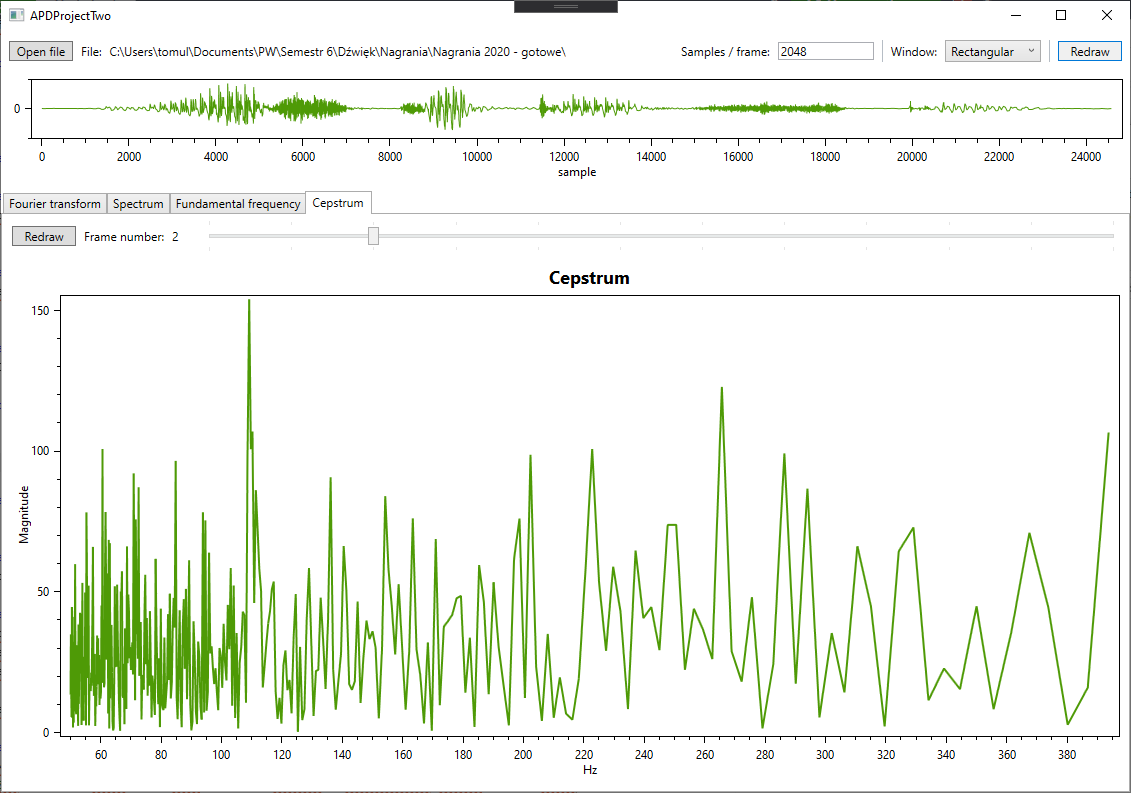
\includegraphics[width=1.0\textwidth]{figures/201_bla_cep}
            \caption{Lektor 201 ``Błaszczykowski'' - cepstrum w okolicy pierwszej samogłoski}
            \label{fig:201_bla_cep}
        \end{figure}


    \subsection{Częstotliwość tonu podstawowego\label{sec:f0}}
        Cepstrum przedstawiane jest w zakresie $[50Hz, 400Hz]$, ponieważ jest to przedział istotny przy znajdowaniu częstotliwości tonu podstawowego. Posiadając już obliczone cepstrum dla każdej ramki, aplikacja liczy następnie zmieniające się w czasie (jednostką czasu jest w tym przypadku ramka) przybliżenie częstotliwości $f_0$ według następującego wzoru:

        \begin{equation*}
            f_0=\frac{1}{\tau_{max}},
        \end{equation*}

        gdzie $\tau_{max}$ wyznaczne z równania

        \begin{equation*}
            C(\tau_{max})=\max_{\tau} C(\tau), \frac{f_s}{\tau} \in [50,400].
        \end{equation*}

        Przykładowy wykres częstotliwości krtaniowej znajduje się na Rys. \ref{fig:201_bla_f0}.

        \begin{figure}[h!]
            \centering
            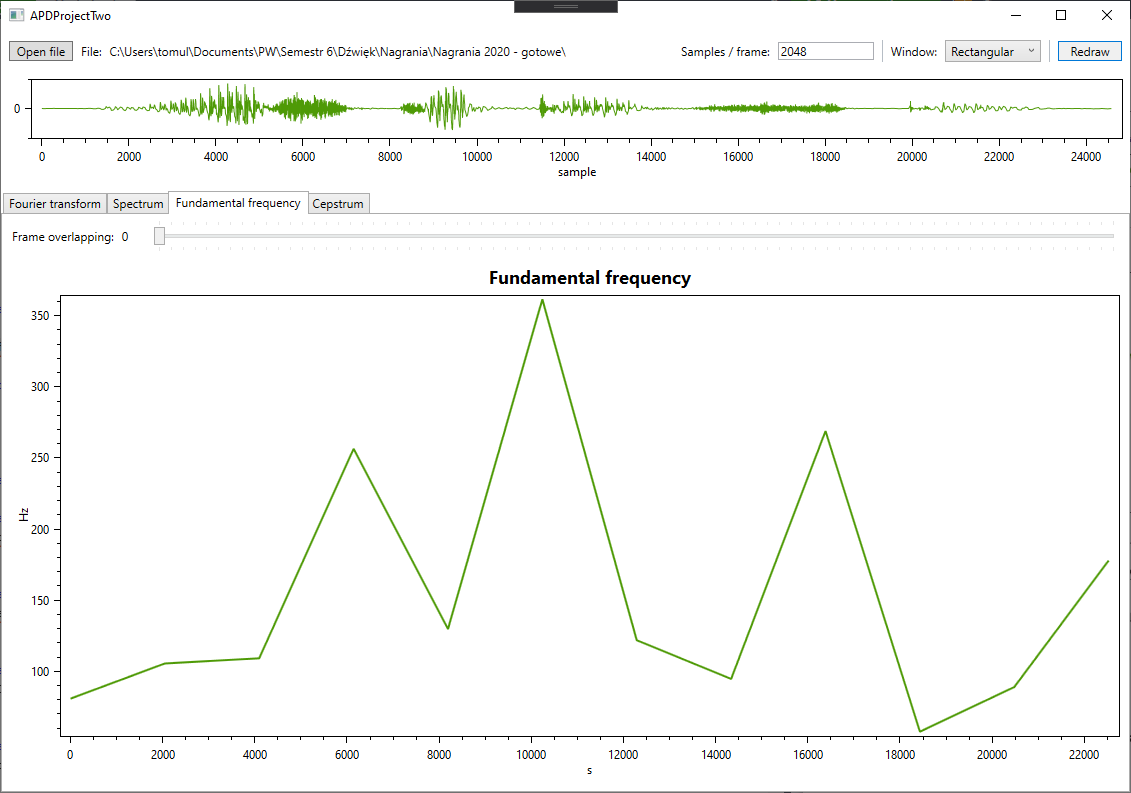
\includegraphics[width=1.0\textwidth]{figures/201_bla_f0}
            \caption{Lektor 201 ``Błaszczykowski'' - częstotliwość krtaniowa}
            \label{fig:201_bla_f0}
        \end{figure}


\section{Wyniki działania\label{sec:prezentacja}}

    \subsection{Formanty}
        Formant – pasmo częstotliwości w dźwięku (np. głosu ludzkiego lub instrumentu muzycznego), w granicach którego wszystkie tony składowe ulegają szczególnemu wzmocnieniu. Zbiór wszystkich formantów danego dźwięku określa jego barwę \cite{drobner53}.

        Z moich obserwacji wynika, że dla pojedynczych lektorów formanty zawsze zostają w podobnej odległości od siebie w realizacjach tego samego fonemu. Na przykład głoska ``a'' lektora 201 zawsze ma formant $F_1$ 1500 Hz i formant $F_2$ w okolicach 2300 Hz. Natomiast różnią się między lektorami. Lektor 204 z niższym głosem niż lektor 201 wykazuje niższe częstotliwości w formantach samogłosek (dla fonemu ``a'' $F_1$ to około 1300 Hz, a $F_2$ to około 1900Hz).


    \subsection{Różnice między spółgłoskami i samogłoskami}
        Jako przykład różnic miedzy spółgłoskami i samogłoskami wybrałem słowo ``skijapapa''. Na spektrogramie (Rys. \ref{fig:skijapapa_201_analiza}) doskonale przedstawiają się kolejne głoski.

        \begin{itemize}
            \item ``s'' charakteryzuje się dużą ilością szumu w wysokich częstotliwościach i brakiem wyraźnego tonu podstawowego,
            \item ``ki'' rozpoczyna się szumem we wszystkich częstotliwościach (głoska ``k''), a nastepnie przechodzi w głoskę ``i'' z charakterystyczną przerwą między tonem podstawowym a wyższymi formantami,
            \item ``ja'' widoczne jest jako płynne przejście (zaznaczone na Rys. \ref{fig:skijapapa_201_analiza} białymi kreskami) pomiędzy formantami widocznymi w ``i'' a formantami widocznymi w ``a'',
            \item ``p'' charakteryzuje się tutaj szumem, widocznym głównie w niższych częstotliwościach z racji następującego po nim ``a'',
            \item ``a'' ma charakterystyczny układ formantów, który został zaznaczony na Rys. \ref{fig:skijapapa_201_analiza} niebieską poziomą linią.
        \end{itemize}

        \begin{figure}[h!]
            \centering
            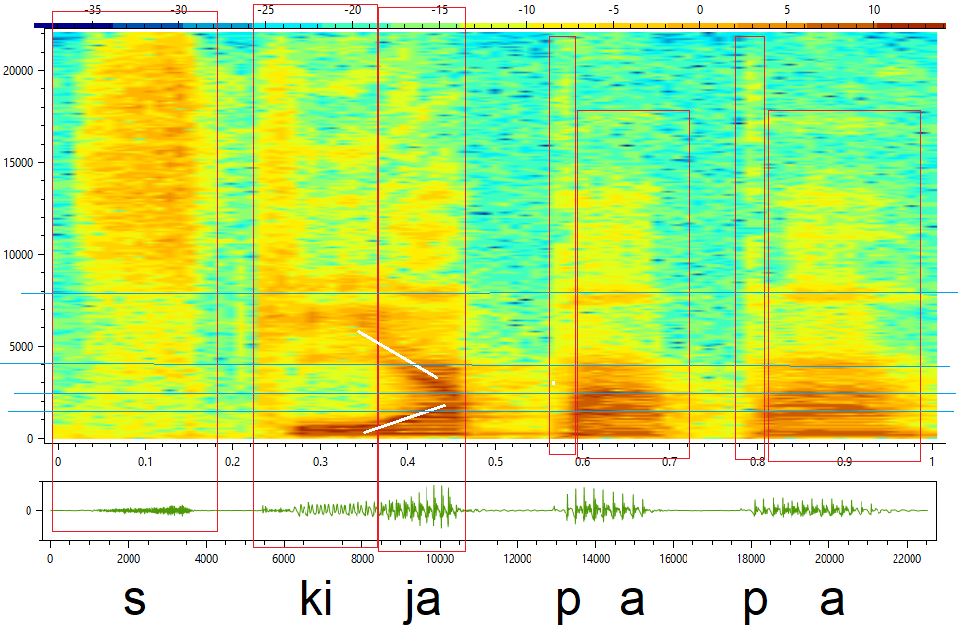
\includegraphics[width=1.0\textwidth]{figures/skijapapa_201_analiza.png}
            \caption{Lektor 201 ``skijapapa'' - analiza spektrogramu}
            \label{fig:skijapapa_201_analiza}
        \end{figure}

        Jak widać spółgłoski bezdźwięczne charakteryzują się dużą ilością szumu różnie rozłożoną na spektrum częstotliwości, a samogłoski - wyklarowanymi formantami, po których można je między sobą rozróżnić. Nie zawsze łatwo jest rozróżnić pojedyncze formanty, dopóki nie wiemy gdzie mniej więcej można się ich spodziewać. Jednak sam fakt, że formanty występują w danej głosce jest zwykle oczywistą wskazówką, że patrzymy na samogłoskę. Znając ``wygląd'' poszczególnych głosek jesteśmy w stanie z dość dużą dokładnością odczytać ze spektrogramu wypowiadane słowo. \cite{russel}


    \subsection{Wpływ funkcji okienkowych}
        Tak jak możnaby się spodziewać, okno kwadratowe wprowadza dużo zakłóceń w wysokich częstotliwościach, natomiast okna Hamminga i Van Hanna potrafią zależnie od sygnału niwelować te zakłócenia mniej lub bardziej. W przykładzie na Rys. \ref{fig:204_kanapka_rect}, \ref{fig:204_kanapka_hamming}, \ref{fig:204_kanapka_vanhann} okno Van Hanna pozostawia najmniej zakłóceń na spektrum.

        \begin{figure}[h!]
            \centering
            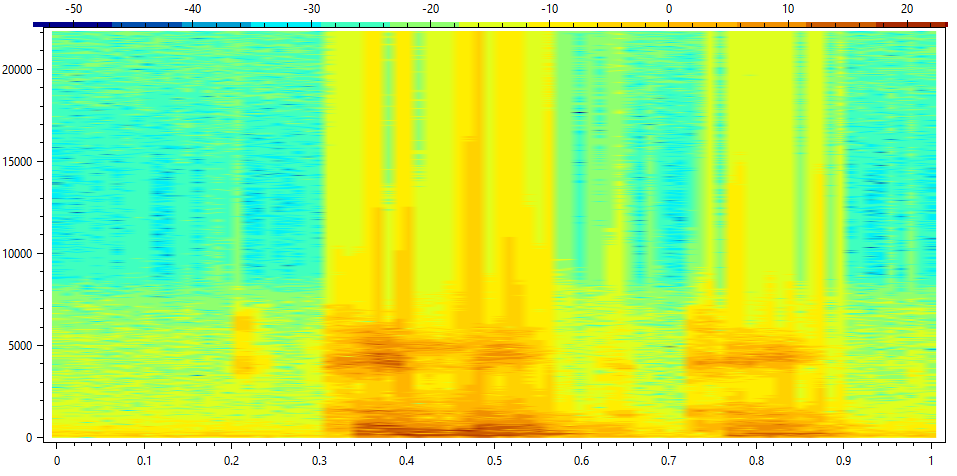
\includegraphics[width=1.0\textwidth]{figures/204_kanapka_rect.png}
            \caption{Lektor 204 ``kanapka'' - okno prostokątne}
            \label{fig:204_kanapka_rect}
        \end{figure}

        \begin{figure}[h!]
            \centering
            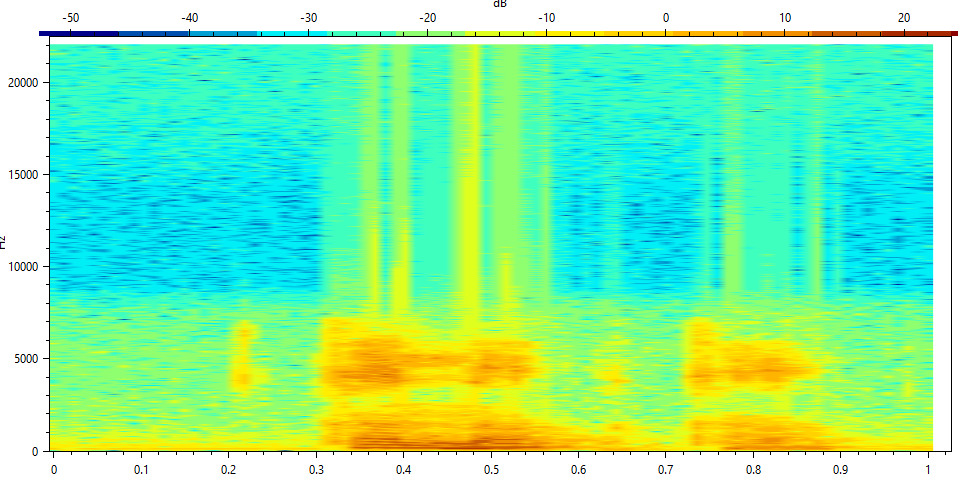
\includegraphics[width=1.0\textwidth]{figures/204_kanapka_hamming.png}
            \caption{Lektor 204 ``kanapka'' - okno Hamminga}
            \label{fig:204_kanapka_hamming}
        \end{figure}

        \begin{figure}
            \centering
            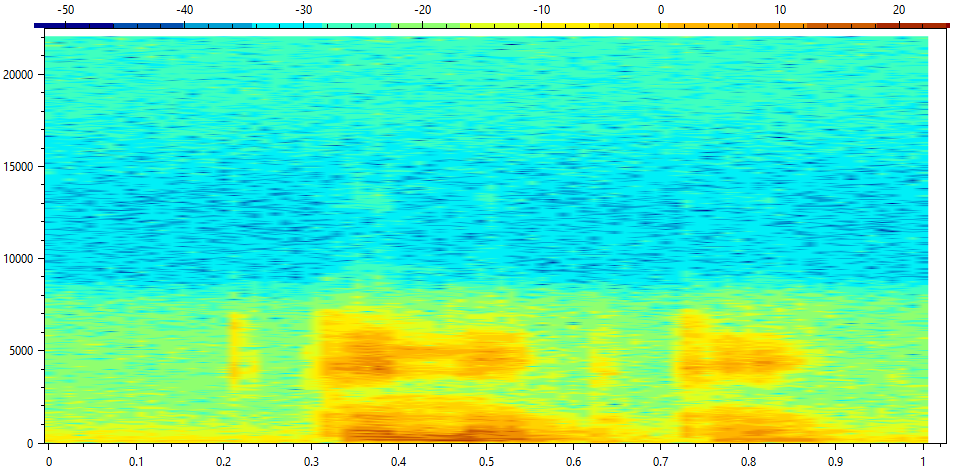
\includegraphics[width=1.0\textwidth]{figures/204_kanapka_vanhann.png}
            \caption{Lektor 204 ``kanapka'' - okno Van Hanna}
            \label{fig:204_kanapka_vanhann}
        \end{figure}


    \subsection{Ton podstawowy }
        Jako przykład działania wybrałem logotom ``aba'' z racji różnorodności intonacji jaką zauważyłem wśród lektorów. Lektor 201 ma na nagraniu intonację opadającą, co widać na malejącym wykresie $f_0$ (Rys. \ref{fig:aba_201_f0}). Lektorzy 203 i 205 mają intonację rosnącą, co widać na rosnących wykresach (Rys. \ref{fig:aba_203_f0} oraz \ref{fig:aba_205_f0}). Natomiast lektor 208 ma stałą intonację, co widoczne jest jako prawie płaski wykres na Rys. \ref{fig:aba_208_f0} (słowo ``aba'' pojawia się około 5100. próbki).

        Można także zauważyć różnicę w zakresie tonów podstawowych. Lektorzy 201 i 208 (Rys. \ref{fig:aba_201_f0} i \ref{fig:aba_208_f0}) to mężczyźni o niższych głosach (odpowiednio $~100Hz$ i $~130Hz$) niż lektorzy 203 i 205 (Rys. \ref{fig:aba_203_f0} i \ref{fig:aba_205_f0}) - kobiety o wyższych głosach (odpowiednio $150-200Hz$ i $250-290Hz$).


        \begin{figure}[h!]
            \centering
            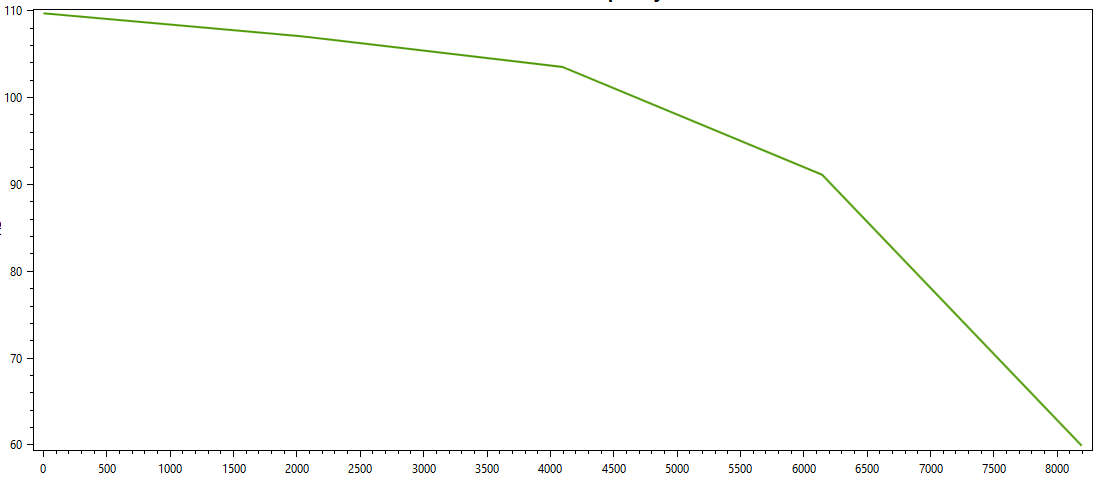
\includegraphics[width=1.0\textwidth]{figures/aba_201_f0.png}
            \caption{Lektor 201 ``aba'' - wykres częstotliwości krtaniowej}
            \label{fig:aba_201_f0}
        \end{figure}

        \begin{figure}[h!]
            \centering
            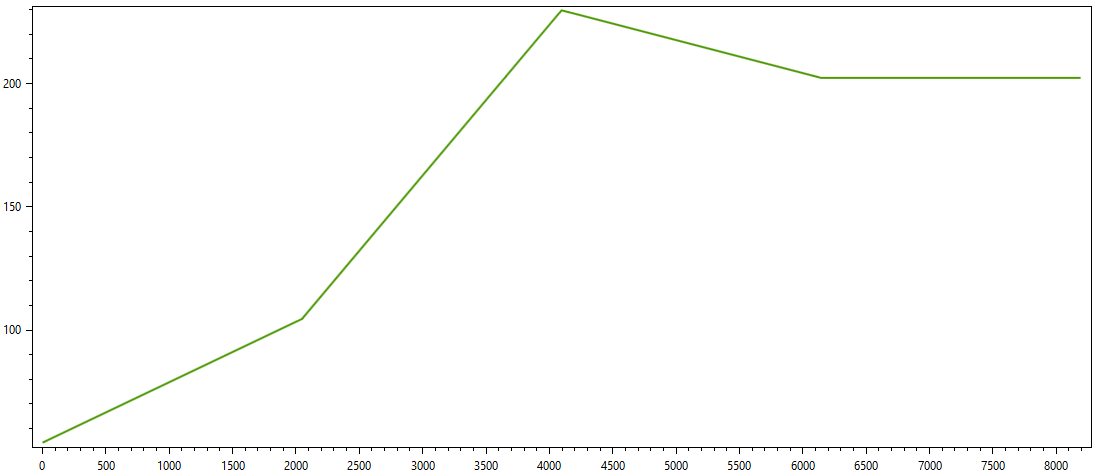
\includegraphics[width=1.0\textwidth]{figures/aba_203_f0.png}
            \caption{Lektor 203 ``aba'' - wykres częstotliwości krtaniowej}
            \label{fig:aba_203_f0}
        \end{figure}

        \begin{figure}[h!]
            \centering
            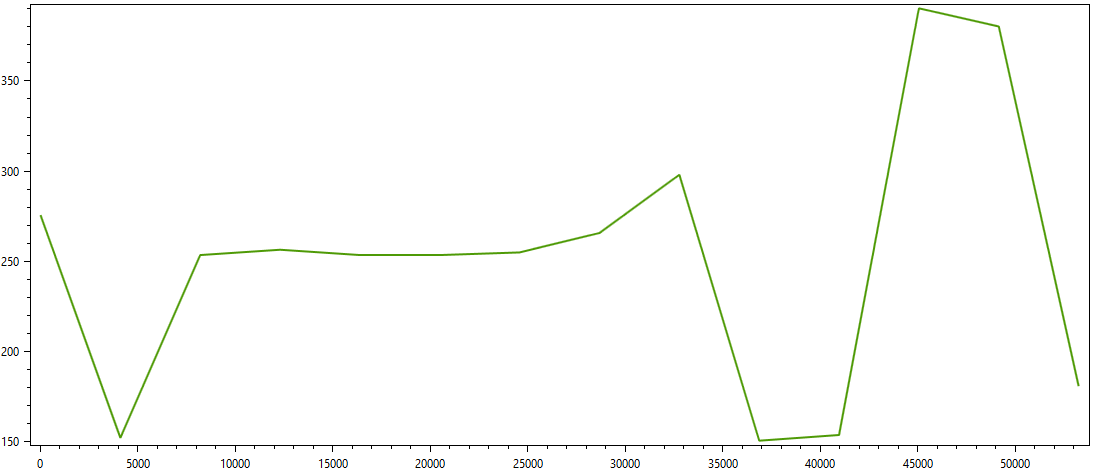
\includegraphics[width=1.0\textwidth]{figures/aba_205_f0.png}
            \caption{Lektor 205 ``aba'' - wykres częstotliwości krtaniowej}
            \label{fig:aba_205_f0}
        \end{figure}

        \begin{figure}[h!]
            \centering
            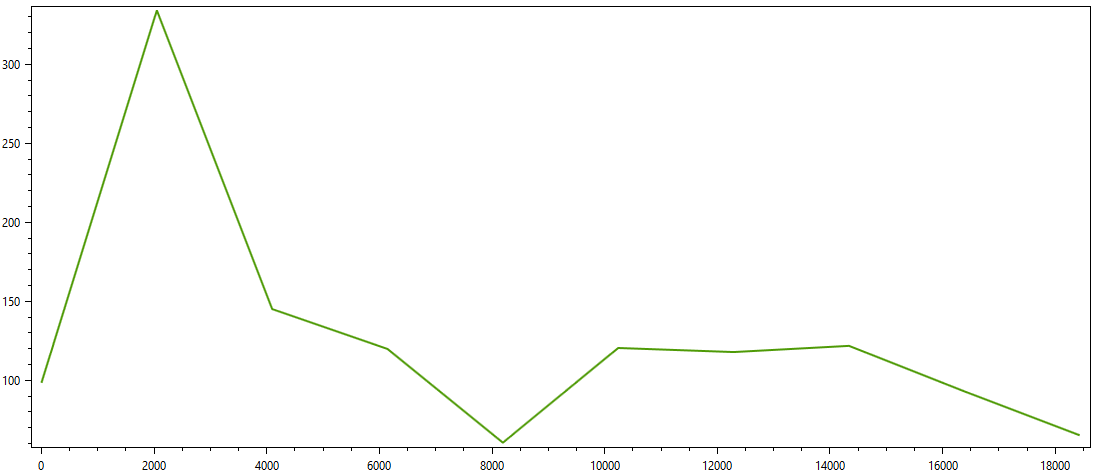
\includegraphics[width=1.0\textwidth]{figures/aba_208_f0.png}
            \caption{Lektor 208 ``aba'' - wykres częstotliwości krtaniowej}
            \label{fig:aba_208_f0}
        \end{figure}

    \clearpage

\section{Wnioski\label{sec:wnioski}}
    Na podstawie wyników i implementacji projektu nasuwają się następujące wnioski:


    \subsection{Czy metody zawsze działają dobrze?\label{sec:czydobrze}}
        Cepstrum wydaje się być dobrą metodą znajdowania częstotliwości krtaniowej w sygnałach dźwiękowych głosu, jednak w wypadku na przykład fal kwadratowych czy trójkątnych nie radzi sobie za dobrze (a przynajmniej moja implementacja).


    \subsection{Modyfikacja parametrów\label{sec:modyfikacja_parametrow}}
        Czasami, aby uzyskać miarodajne wyniki należy dokładnie manipulować parametrami. W szczególności długość ramki i funkcja okna muszą być odpowiednio dobrane. Współczynnik nakładania ramek również bywa pomocny w odsiewaniu ``zaszumionych'' wyników.


    \subsection{Wnioski natury technicznej\label{sec:problemy}}
        Nieporządne implementacje metod numerycznych takich jak transformata Fouriera potrafią wskazywać wyniki dalekie od prawdy w niektórych specyficznych sytuacjach. Na szczęscie implementecje w bibliotece \emph{Math.NET Numerics} nie powodują takich problemów.


\bibliographystyle{plain}
\bibliography{references}

\end{document}
